\documentclass{article}

\usepackage[UTF8]{ctex}
\usepackage[usenames,dvipsnames]{color} 
\usepackage{amsmath}
\usepackage{amssymb}
\usepackage[all]{xy}
\usepackage{geometry}
\usepackage{enumerate}
\usepackage{bm}
\geometry{a4paper,left=3cm,right=3cm,top=3cm,bottom=3cm}
\usepackage[colorlinks,urlcolor=Periwinkle]{hyperref}
\usepackage{tikz}

\newcommand{\E}{\mathrm{E}}
\newcommand{\Var}{\mathrm{Var}}
\newcommand{\Cov}{\mathrm{Cov}}
\newcommand{\y}{\mathbf{y}}
\newcommand{\X}{\mathbf{X}} 
\newcommand{\M}{\mathbf{M}} 
\newcommand{\e}{\mathbf{e}} 
\newcommand{\0}{\mathbf{0}} 
\newcommand{\vbe}{\bm{\beta}}   
\newcommand{\vep}{\bm{\varepsilon}}  
\newcommand{\vb}{\mathbf{b}} 
\newcommand{\pro}{\noindent$\vartriangleright\,$\textbf{问题}.\ }
\newcommand{\sol}{\noindent$\vartriangleright\,$\textbf{解答}.\ }

\begin{document}

\noindent{\huge \textbf{Problem Set}}\\ 

\section{Finite-Sample Properties of OLS}

\subsection{新增样本点}
\pro 给定简单线性模型
\[
\y = \X \vbe +\vep,
\]
其中 
\[
\y=(y_1,\cdots,y_n)',\;\X=
\begin{pmatrix}
1& x_1\\
1& x_2\\
\vdots&\vdots\\
1& x_n
\end{pmatrix},\;
\vbe=(\beta_0,\beta_1)',\;
\vep=(\varepsilon_1,\cdots,\varepsilon_n)'.
\]
设该模型在 Gauss-Markov 假设下,OLS 估计量为 $\vb=(b_0,b_1)'$. 若新增一个样本点
\[
y_{n+1}=\beta_0+\beta_1x_{n+1}+\varepsilon_{n+1},
\]
求 $\Var(\hat{y}_{n+1}-y_{n+1}|\X,x_{n+1})$,其中 $\hat{y}_{n+1}=b_0+x_{n+1}b_1$. 在给定 $\X$ 的情况下,求出当 $x_{n+1}$ 为何值时, $\Var(\hat{y}_{n+1}-y_{n+1}|\X,x_{n+1})$ 有最小值.\\


\sol
\begin{align*}
\hat{y}_{n+1}-y_{n+1}&=(b_0+x_{n+1}b_1)-(\beta_0+x_{n+1}\beta_1+\varepsilon_{n+1})\\
&=(b_0-\beta_0)+x_{n+1}(b_1-\beta_1)-\varepsilon_{n+1}
\end{align*}
记 $\bar{x}=n^{-1}\sum_{i=1}^{n}x_i$. 因为
\begin{align*}
\Var(\vb|\X,x_{n+1})&=\sigma^2(\X'\X)^{-1}=\sigma^2
\begin{pmatrix}
n& \sum\limits_{i=1}^{n}x_i\\
\sum\limits_{i=1}^{n}x_i& \sum\limits_{i=1}^{n}x_i^2
\end{pmatrix}^{-1}\\
&=\frac{\sigma^2}{\sum\limits_{i=1}^{n}(x_i-\bar{x})^2}
\begin{pmatrix}
n^{-1}\sum\limits_{i=1}^{n}x_i^2& -\bar{x}\\
 -\bar{x}& 1
\end{pmatrix}.
\end{align*}
所以
\[
\Var(b_0-\beta_0|\X,x_{n+1})=\frac{\sigma^2\sum\limits_{i=1}^{n}x_i^2}{n\sum\limits_{i=1}^{n}(x_i-\bar{x})^2},
\]
\[
\Var[x_{n+1}(b_1-\beta_1)|\X,x_{n+1}]=\frac{\sigma^2x_{n+1}^2}{\sum\limits_{i=1}^{n}(x_i-\bar{x})^2},
\]
\[
\Var(\varepsilon_{n+1}|\X,x_{n+1})=\sigma^2,
\]
\[
\Cov[b_0-\beta_0,x_{n+1}(b_1-\beta_1)|\X,x_{n+1}]=-\frac{\sigma^2\bar{x}x_{n+1}}{\sum\limits_{i=1}^{n}(x_i-\bar{x})^2},
\]
\[
\Cov(b_0-\beta_0,\varepsilon_{n+1}|\X,x_{n+1})=\Cov[x_{n+1}(b_1-\beta_1),\varepsilon_{n+1}|\X,x_{n+1}]=0.
\]
由此可得
\begin{align*}
\Var(\hat{y}_{n+1}-y_{n+1}|\X,x_{n+1})&=\frac{\sigma^2\sum\limits_{i=1}^{n}x_i^2+n\sigma^2x_{n+1}^2-2n\sigma^2\bar{x}x_{n+1}}{n\sum\limits_{i=1}^{n}(x_i-\bar{x})^2}+\sigma^2\\
&=\frac{\sigma^2}{\sum\limits_{i=1}^{n}(x_i-\bar{x})^2}\left(x_{n+1}^2-2\bar{x}x_{n+1}+\frac{1}{n}\sum\limits_{i=1}^{n}x_i^2\right)+\sigma^2.
\end{align*}
当 $x_{n+1}=\bar{x}$ 时,$\Var(\hat{y}_{n+1}-y_{n+1}|\X,x_{n+1})$ 有最小值.

\subsection{增加解释变量个数会提高 $R^2$}
\pro 证明对简单线性模型
\[
\y_{n\times1} = \X_{n\times K} \vbe_{K\times1} +\vep_{n\times1}, 
\]
进行 OLS 回归时,使用 $K-1$ 个解释变量的 $R^2$ 小于等于使用 $K$ 个解释变量时的 的 $R^2$.\\

\sol
使用 $K$ 个自变量时,OLS 估计量 $\vb$ 最小化了残差平方和
\[
\vb=\arg\min_{\hat{\vbe}\in\mathbb{R}^K}\Vert\y-\X\hat{\vbe}\Vert^2.
\]
因此,对任意 $\hat{\vbe}\in\mathbb{R}^K$, 有
\[
\Vert\y-\X\hat{\vbe}\Vert^2\ge\Vert\y-\X\vb\Vert^2=SSR_K.
\]
设使用 $K-1$ 个自变量时对应的 OLS 估计量为 $\vb_{-K}\in\mathbb{R}^{K-1}$. 令 $\vb_{-K}^*=(\vb_{-K},0)$, 利用上式得到
\[
SSR_{K-1}=\Vert\y-\X\vb_{-K}\Vert^2=\Vert\y-\X\vb_{-K}^*\Vert^2\ge SSR_K.
\]
由 $R^2$ 的表达式
\[
R^2=1-\frac{SSR}{\sum\limits_{i=1}^n(y_i-\bar{y})^2}
\]    
可知使用 $K-1$ 个解释变量的 $R^2$ 小于等于使用 $K$ 个解释变量时的 的 $R^2$. 该结果的几何解释如下图所示.
\[
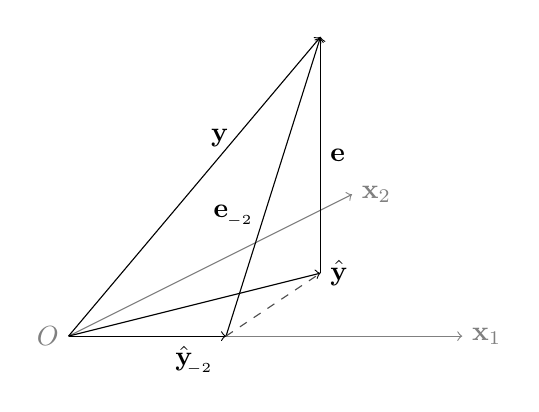
\begin{tikzpicture}
\draw [color=black!50,->](0,0) node[left]{$O$}-- node [color=black!20,pos=0.25,above,sloped]{}(3.6,1.8) node[right]{$\mathbf{x}_2$};
\draw [color=black!50,->](0,0) node[left]{}-- node [color=black!20,pos=0.25,above,sloped]{}(5,0) node[right]{$\mathbf{x}_1$};
\draw [color=black,->](0,0) node[left]{}-- node [color=black,pos=0.6,above]{$\y$}(3.2,3.8) node[right]{};
\draw [color=black,->](3.2,0.8) node[left]{}-- node [color=black,pos=0.5,right]{$\e$}(3.2,3.8) node[right]{};
\draw [color=black,->](0,0) node[left]{}-- node [color=red!70,pos=0.25,above,sloped]{}(3.2,0.8) node[right]{$\hat{\y}$};
\draw [color=black,->](2,0) node[left]{}-- node [color=black,pos=0.4,left]{$\e_{\hspace{-0.5pt}_{-2}}$}(3.2,3.8) node[right]{};
\draw [color=black,->](0,0) node[left]{}-- node [color=black,pos=0.8,below]{$\hat{\y}_{\hspace{-2pt}_{-2}}$}(2,0) node[right]{};
\draw [color=black!70,-,dashed](2,0) node[left]{}-- node [color=red!70,pos=0.25,above,sloped]{}(3.2,0.8) node[right]{};
\end{tikzpicture}
\]
这幅图展示了 $K=2$ 的低维情形,其中 $\mathbf{x}_1$, $\mathbf{x}_2$ 是 $\X$ 的列向量,$\e=\y-\X\vb$. 根据直角三角形的斜边长度大于直角边这一性质可以得到
\[
SSR_{1}=\Vert\e_{-2}\Vert^2\ge\Vert\e\Vert^2= SSR_2.
\] 
除非 $\y$ 在 $\mathbf{x}_2$ 上的投影为 0,以上不等式严格成立。沿着这个思路,我们可以给出另一种证明。因为
\[
\Vert\e_{-K}\Vert^2=\Vert(\e_{-K}-\e)+\e\Vert^2=\Vert\e_{-K}-\e\Vert^2+\Vert\e\Vert^2+2(\e_{-K}-\e)'\e,
\]
故只需证明 $(\e_{-K}-\e)'\e=0$. 设使用 $K$ 个自变量时回归时,零化子 $\M=\mathbf{I}_n-\X(\X'\X)^{-1}\X'$,使用 $K-1$ 个自变量时对应的零化子为 $\M_{-K}=\mathbf{I}_{n}-\X_{-K}(\X_{-K}'\X_{-K})^{-1}\X_{-K}'$. 注意到
\[
\X'\e=\0_{K\times 1}\implies\X'_{K-1}\e=\0_{(K-1)\time 1},
\]
我们有
\begin{align*}
(\e_{-K}-\e)'\e=(\y'\M'_{-K}-\y'\M')\e=\y'(\M'_{-K}\e-\M'\e).
\end{align*}
一方面,
\[
\M'_{-K}\e=(\mathbf{I}_{n}-\X_{-K}(\X_{-K}'\X_{-K})^{-1}\X_{-K}')\e=\e,
\]
另一方面,
\[
\M'\e=\M\M\y=\M\y=\e,
\]
故可得
\[
(\e_{-K}-\e)'\e=\y'(\e-\e)=0.
\]
于是我们证明了
\[
\Vert\e_{-K}\Vert^2=\Vert\e_{-K}-\e\Vert^2+\Vert\e\Vert^2\ge\Vert\e\Vert^2.
\]

\subsection{模型误设:加入无关变量}
\pro 已知 DGP(数据生成过程)
\[
\y = \underset{(n\times K_1)}{\X_1}\vbe_1 +\vep.
\]
若使用如下模型进行估计
\[
\y = \underset{(n\times K_1)}{\X_1} \vbe_1 +\underset{(n\times K_2)}{\X_2} \vbe_2+\vep^*,
\]
将得到对应的 OLS 估计量 $\vb=(\vb_1,\vb_2)$. 在 Gauss-Markov 假定满足的条件下,证明 $\E[\vb_1|\X_1,\X_2]=\vbe_1$,$\Var[\vb_1|\X_1,\X_2]\ge\sigma^2(\X_1'\X_1)^{-1}$.\\

\sol 设 $\M=\mathbf{I}_n-\X(\X'\X)^{-1}\X'$,$\M_2=\mathbf{I}_n-\X_2(\X_2'\X_2)^{-1}\X_2'$. 用 $\X'_1\M_2$ 左乘
\[
\y = \X_1\vb_1 +\X_2 \vb_2+\e.
\]
得到
\begin{equation}
	\X'_1\M_2\y = \X'_1\M_2\X_1\vb_1 +\X'_1\M_2\X_2 \vb_2+\X'_1\M_2\e.
\end{equation}
因为 $\X'\e=\0\implies\X_1'\e=\X_2'\e=\0$,类似 1.2 可以得到
\[
\M_2\e=(\mathbf{I}_n-\X_2(\X_2'\X_2)^{-1}\X_2')\e=\e-\X_2(\X_2'\X_2)^{-1}\X_2'\e=\e,
\]
从而有 $\X'_1\M_2\e=\X'_1\e=\0$. 又由 $\M_2\X_2=\0$ 知 $\X'_1\M_2\X_2 \vb_2=\0$. 于是 (1) 式简化为
\[
\X'_1\M_2\y = \X'_1\M_2\X_1\vb_1 .
\]
为证明 $\X'_1\M_2\X_1$ 可逆,我们可以使用反证法. 设矩阵 $\X'_1\M_2\X_1$ 的秩小于 $K_1$,则存在非零向量 $\mathbf{v}\in\mathbb{R}^{K_1}$,使得
\[
\X'_1\M_2\X_1\mathbf{v}=\mathbf{0},
\]
从而有
\[
\mathbf{v}'\X'_1\M_2\X_1\mathbf{v}=(\M_2\X_1\mathbf{v})'(\M_2\X_1\mathbf{v})=0\implies \M_2\X_1\mathbf{v}=\mathbf{0}.
\]
由 $\M_2\X_2=\0$ 知 $\mathrm{Im}\X_2\subseteq\mathrm{Ker}\M_2$. 注意到 $\dim\mathrm{Im}\X_2=\dim\mathrm{Ker}\M_2=K_2$,因此有 $\mathrm{Im}\X_2=\mathrm{Ker}\M_2$. 故存在 $\mathbf{w}\in\mathbb{R}^{K_1}$,使得 \[
\X_1\mathbf{v}=\X_2\mathbf{w}\in\mathrm{Im}\X_1\cap\mathrm{Im}\X_2.
\]
由 $\X_{1}$ 列满秩知 $\X_1\mathbf{v}\ne\mathbf{0}$,故 $\dim(\mathrm{Im}\X_1\cap\mathrm{Im}\X_2)\ge1$,从而
\[
\dim(\mathrm{Im}\X_1\cup\mathrm{Im}\X_2)=\dim\mathrm{Im}\X_1+\dim\mathrm{Im}\X_2-\dim(\mathrm{Im}\X_1\cap\mathrm{Im}\X_2)\le K_1+K_2-1,
\]
这与 $(\X_1,\X_2)$ 列满秩矛盾!这样就证明了 $\X'_1\M_2\X_1$ 可逆. 由此解出
\[
\vb_1=(\X'_1\M_2\X_1)^{-1}\X'_1\M_2\y.
\]
于是我们可以将 $\vb_1-\vbe_1$ 表示成 $\X_1$,$\X_2$ 和 $\vep$ 的函数
\begin{align*}
\vb_1-\vbe_1&=(\X'_1\M_2\X_1)^{-1}\X'_1\M_2\y-\vbe_1\\
&=(\X'_1\M_2\X_1)^{-1}\X'_1\M_2(\X\vbe_1+\vep)-\vbe_1\\
&=(\X'_1\M_2\X_1)^{-1}\X'_1\M_2\X\vbe_1+(\X'_1\M_2\X_1)^{-1}\X'_1\M_2\vep-\vbe_1\\
&=\vbe_1+(\X'_1\M_2\X_1)^{-1}\X'_1\M_2\vep-\vbe_1\\
&=(\X'_1\M_2\X_1)^{-1}\X'_1\M_2\vep\\
&=\mathbf{C}\vep\qquad(\text{令 } \mathbf{C}=(\X'_1\M_2\X_1)^{-1}\X'_1\M_2).
\end{align*}
故
\[
\E[\vb_1-\vbe_1|\X_1,\X_2]=\E[\mathbf{C}\vep|\X_1,\X_2]=\mathbf{C}\E[\vep|\X_1,\X_2]=0,
\]
即 $\E[\vb_1|\X_1,\X_2]=\vbe_1$. 下面证明一个引理:设 $\mathbf{A},\mathbf{B}$ 正定,
\[
\mathbf{A}\ge\mathbf{B}\implies\mathbf{B}^{-1}\ge\mathbf{A}^{-1}.
\]
事实上,这可由恒等式
\[
\mathbf{B}^{-1}-\mathbf{A}^{-1} = \mathbf{A}^{-1}(\mathbf{A}-\mathbf{B})\mathbf{A}^{-1}
=\mathbf{A}^{-1}(\mathbf{A}-\mathbf{B})\mathbf{A}^{-1} + \mathbf{A}^{-1}(\mathbf{A}-\mathbf{B})\mathbf{B}^{-1}(\mathbf{A}-\mathbf{B})\mathbf{A}^{-1}
\]
直接得到. 因为
\begin{align*}
\Var[\vb_1|\X_1,\X_2]&=\Var[\vb_1-\vbe_1|\X_1,\X_2]\\
&=\Var[\mathbf{C}\vep|\X_1,\X_2]\\
&=\mathbf{C}\Var[\vep|\X_1,\X_2]\mathbf{C}'\\
&=\sigma^2(\X'_1\M_2\X_1)^{-1}\X'_1\M_2\M_2'\X_1(\X'_1\M_2'\X_1)^{-1}\\
&=\sigma^2(\X'_1\M_2\X_1)^{-1},
\end{align*}
要证明
\[
\sigma^2(\X'_1\M_2\X_1)^{-1}\ge\sigma^2(\X_1'\X_1)^{-1},
\]
只需证明
\[
\X_1'\X_1\ge\X'_1\M_2\X_1.
\]
设投影矩阵 $\mathbf{P}_2=\X_2(\X_2'\X_2)^{-1}\X_2'=\mathbf{I}_n-\M$,则只需证
\[
\X_1'\mathbf{P}_2\X_1=(\mathbf{P}_2\X_1)'(\mathbf{P}_2\X_1)\ge\mathbf{O}.
\]
上式确实成立,因此我们证明了 $\Var[\vb_1|\X_1,\X_2]\ge\sigma^2(\X_1'\X_1)^{-1}$.

\subsection{模型误设:遗漏变量}
\pro 已知 DGP(数据生成过程)
\[
\y = \underset{(n\times K_1)}{\X_1} \vbe_1 +\underset{(n\times K_2)}{\X_2} \vbe_2+\vep
\]
若使用如下模型进行估计
\[
\y = \underset{(n\times K_1)}{\X_1}\vbe_1 +\vep^*.
\]
证明 $\E[\vb_1|\X_1]\neq\vbe_1$,并说明等号何时成立.\\
\sol 易得
\begin{align*}
\vb_1&=(\X'_1\X_1)^{-1}\X'_1\y\\
&=(\X'_1\X_1)^{-1}\X'_1(\X_1\vbe_1+\X_2\vbe_2+\vep)\\
&=\vbe_1+(\X'_1\X_1)^{-1}\X_2\vbe_2+(\X'_1\X_1)^{-1}\vep
\end{align*}
故
\begin{align*}
\E[\vb_1|\X_1]&=\E[\vbe_1+(\X'_1\X_1)^{-1}\X_2\vbe_2+(\X'_1\X_1)^{-1}\vep|\X_1]\\
&=\vbe_1+\E[(\X'_1\X_1)^{-1}\X_2\vbe_2|\X_1]\\
&=\vbe_1+(\X'_1\X_1)^{-1}\E[\X_2|\X_1]\vbe_2\\
&\neq\vbe_1
\end{align*}
显然,等号成立当且仅当$\E[\X_2|\X_1]=0$.
\end{document}